\chapter{Multiple Assets with Multiple Volatility Factors}
\miniabstract{The preceding experiment traded one asset whose volatility had six factors. We now trade two assets, each with six factors, and let each quote depend on both inventories. A transparent covariance correction reduces average integrated risk in the first experiment, but also lowers mean PnL. It is a baseline extension, not yet the fitted residual correction proposed in this paper.}

\section{Two inventories, twelve volatility states}
Asset dimension and factor dimension have different roles. The inventory vector is $q=(q_A,q_B)$: it counts the two instruments that can be bought or sold. The volatility state is
\[
 Z=(Z_{A,1},\ldots,Z_{A,6},Z_{B,1},\ldots,Z_{B,6}).
\]
Its twelve coordinates describe persistent and rapidly decaying volatility components. They are not twelve tradable assets. Each asset has its own aggregate $Y_i=\sum_{m=1}^6w_mZ_{i,m}$ and volatility $\sigma_i(Y_i)$.

The two lifts use the same six rates, geometrically spaced between 3 and 180, with normalized weights $w_m\propto\lambda_m^{-0.7}$. Their marginal parameters match the existing scalar export, permitting reuse of its lookup tables without an additional calibration claim. The processes are
\[
 dZ_{i,m}=-\lambda_m Z_{i,m}\,dt+dB_i,
 \qquad d\langle B_A,B_B\rangle_t=\nu\,dt,\quad \nu=0.35.
\]
Within an asset, the six factors share a Brownian driver but filter its history at different rates. Across assets, the drivers are correlated rather than identical. Conditional price dynamics are
\[
 dS_i=\sigma_i(Y_i)\,dW_i,\qquad
 d\langle W_A,W_B\rangle_t=\rho\,dt,\quad \rho=0.7,
\]
with the price Brownian vector independent of the volatility Brownian vector. Thus $\nu$ controls common volatility shocks, whereas $\rho$ controls contemporaneous price shocks. Neither is inferred from the other. We retain
\[
 \sigma_i(Y_i)=1.1\exp\!\left[\frac12\left(0.75Y_i-
 \frac{0.75^2}{2}\operatorname{Var}(Y_i)\right)\right].
\]
The instantaneous covariance of price changes is
\[
 \Sigma(Y)=\begin{pmatrix}
 \sigma_A^2 & \rho\sigma_A\sigma_B\\
 \rho\sigma_A\sigma_B & \sigma_B^2
 \end{pmatrix}.
\]
Here $\rho$ is constant but $\Sigma$ is stochastic. This is not a stochastic-correlation model. Figure~\ref{fig:multi-vol} separates the twelve factor paths from the resulting two volatilities and the covariance. Assets A and B are synthetic; the experiment does not estimate the correlation of any actual pair of companies.

\begin{figure}[htbp]
\centering
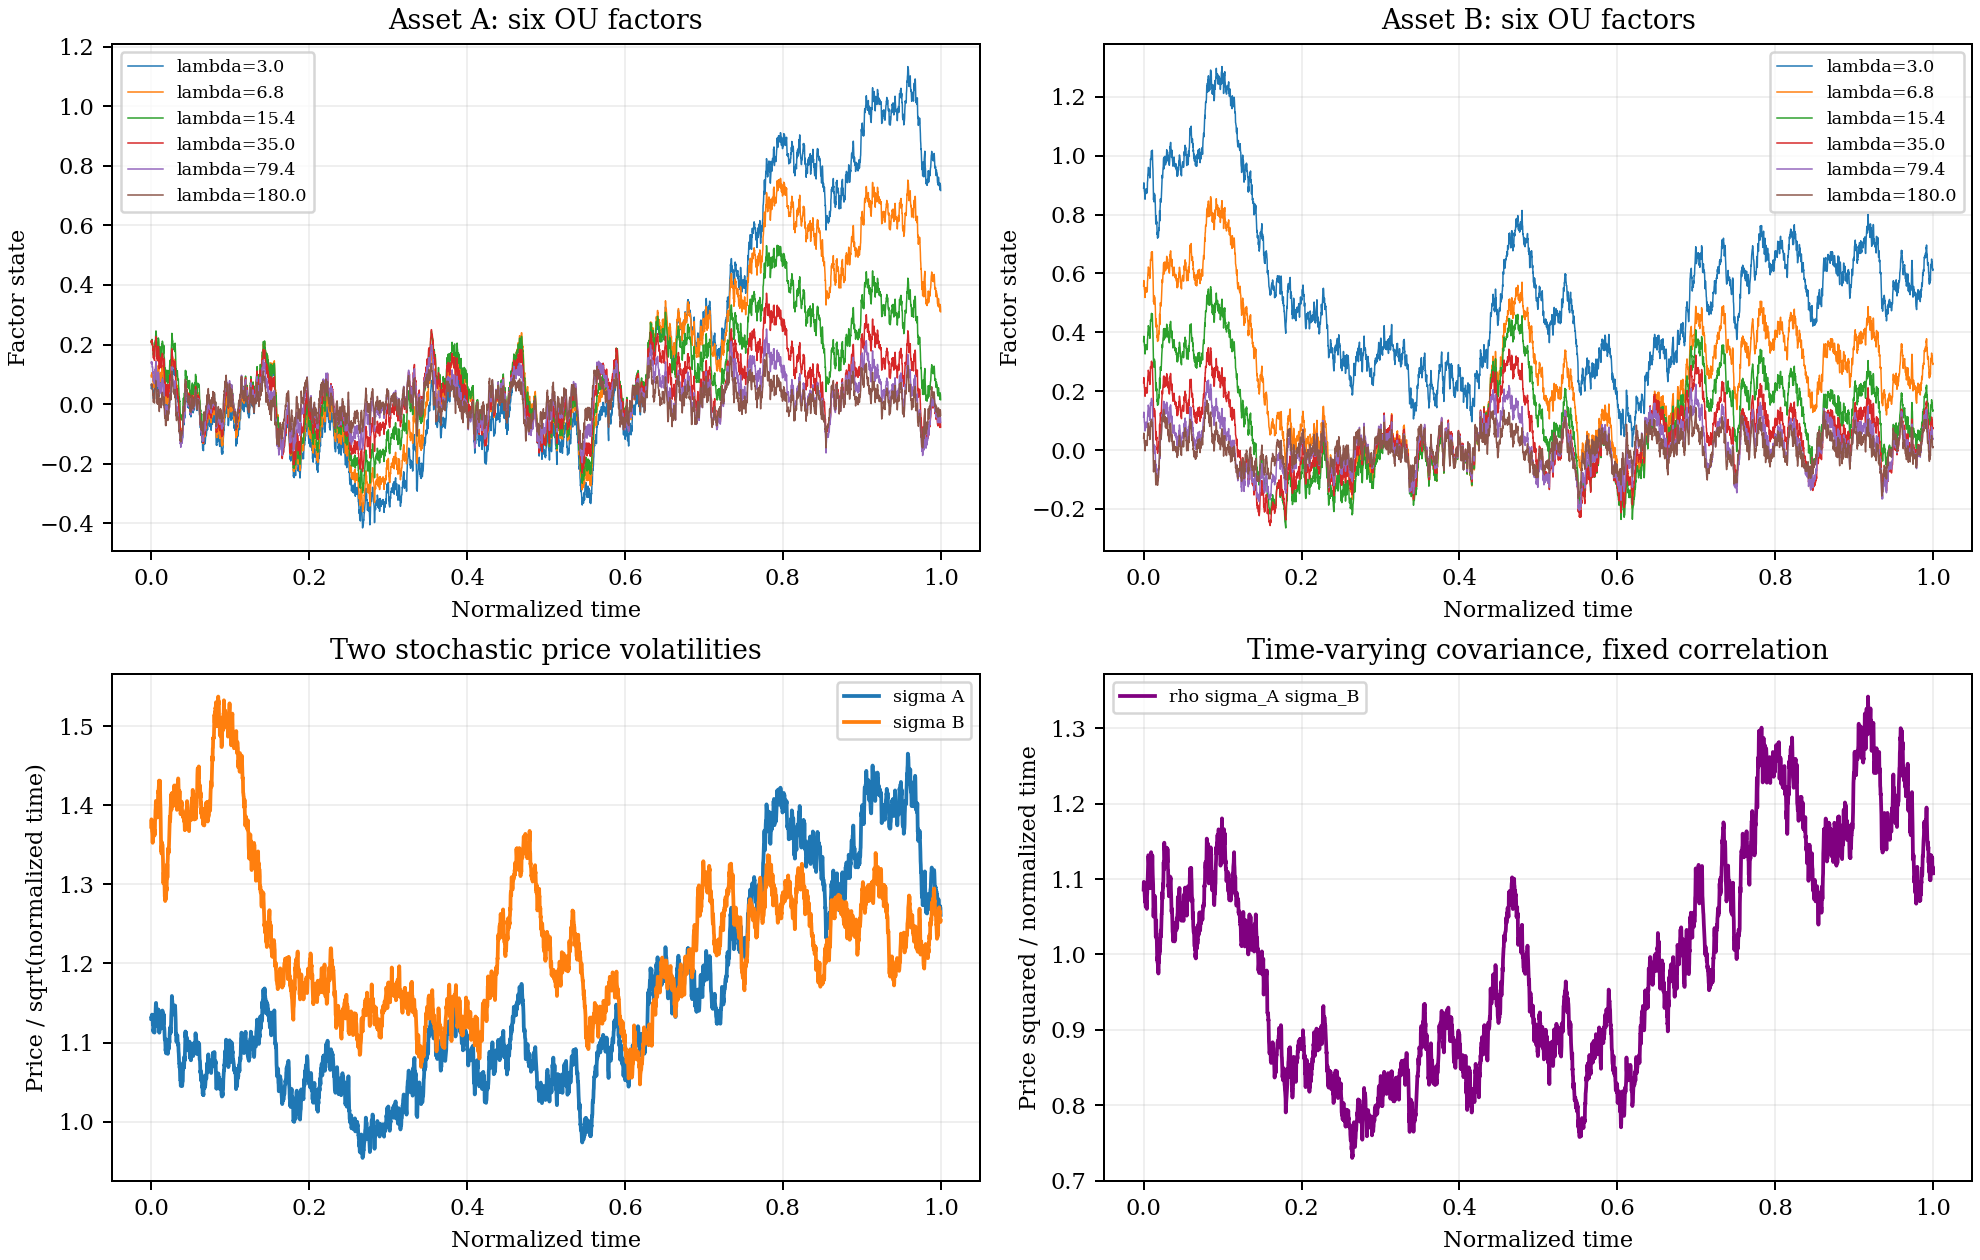
\includegraphics[width=\textwidth]{img/multiasset_volatility.png}
\caption{Two assets with six volatility factors each. Top panels show the two lifts; bottom panels show their distinct price volatilities and $\Sigma_{AB}=\rho\sigma_A\sigma_B$. Seed 73, path zero, stationary initial factor distribution, 3900 time intervals. Equal marginal parameters do not imply equal realized volatility paths.}
\label{fig:multi-vol}
\end{figure}

Exact innovations for the twelve-dimensional lift use
\[
 Q_{(i,m),(j,n)}=\nu_{ij}
 \frac{1-e^{-(\lambda_m+\lambda_n)\Delta t}}{\lambda_m+\lambda_n},
 \qquad \nu_{AA}=\nu_{BB}=1,\quad \nu_{AB}=0.35.
\]
The covariance is nearly singular for small steps. A spectral factorization removes only negative eigenvalues attributable to rounding, with a guard against a materially indefinite matrix. The maximum reconstruction discrepancy in the main run is $9.76\times10^{-19}$. This validates the factorization arithmetic, not the complete simulation discretization.

\section{How another asset's inventory changes a quote}
The variance rate of marked portfolio wealth is
\[
 \mathcal V(q,Y)=q^\top\Sigma(Y)q
 =q_A^2\sigma_A^2+q_B^2\sigma_B^2
 +2q_Aq_B\rho\sigma_A\sigma_B.
\]
With positive correlation, opposite-sign positions make the cross term negative. A short B position can therefore offset part of a long A exposure. The relevant object is this total risk, not the absolute inventory of either asset alone. For a unit sale of B, the exact change at fixed covariance is
\[
 \mathcal V(q-e_B,Y)-\mathcal V(q,Y)
 =-2(\Sigma q)_B+\Sigma_{BB}.
\]
Consequently the next sale reduces instantaneous risk only when $(\Sigma q)_B>\Sigma_{BB}/2$. The covariance benefit does not justify unlimited shorting. Finite order size, own-asset exposure, bounds and liquidation all matter. For example, at equal unit volatilities and $\rho=0.7$, moving from $(3,0)$ to $(3,-1)$ reduces the variance rate from 9 to 5.8; moving from $(3,-6)$ to $(3,-7)$ instead increases it, even before enforcing the inventory limit.

Multi-asset quoting and computational approximations are established research directions~\cite{multiapprox,multifactor}. To isolate the mechanism with our existing numerical baseline, start from the separable value
\[
 \theta_{\rm sep}(t,q,Y)
 =\theta_0(t,q_A,Y_A)+\theta_0(t,q_B,Y_B).
\]
It ignores cross-asset inventory risk in its quote calculation. The first explicit correction is
\[
 C_{\rm cov}(t,q,Y)=-\gamma(T-t)\Sigma_{AB}(Y)q_Aq_B,
 \qquad \theta_{\rm cov}=\theta_{\rm sep}+C_{\rm cov}.
\]
This approximates the omitted integrated cross-risk by freezing the current covariance over the remaining horizon. It is not an exact expectation of future covariance, and it does not solve the joint control problem. It vanishes at $T$, preserving the separable terminal liquidation cost.

Define $s_B=\gamma(T-t)\Sigma_{AB}q_A$. Buying one unit of B changes the correction by $-s_B$, while selling one changes it by $+s_B$. Since the unbounded optimal offset equals the zero-gain offset minus the neighboring-inventory gain, the implementation adds $s_B$ to the raw bid offset and subtracts $s_B$ from the raw ask offset, then applies the declared bounds. Asset A uses the symmetric expression $s_A=\gamma(T-t)\Sigma_{AB}q_B$. Applying the correction before clipping avoids losing the original gain when the baseline control is already at a bound.

If $q_A>0$ and $\rho>0$, the B ask can therefore move downward relative to the separate policy: the dealer accepts a lower selling price because the fill can offset portfolio exposure. Its B bid also moves downward, discouraging further purchases. This is a change relative to the separate quote, not a promise to sell below the mid-price, nor a guaranteed execution. Figure~\ref{fig:multi-shift} makes the sign change with correlation and inventory visible while holding all other inputs fixed.

\begin{figure}[htbp]
\centering
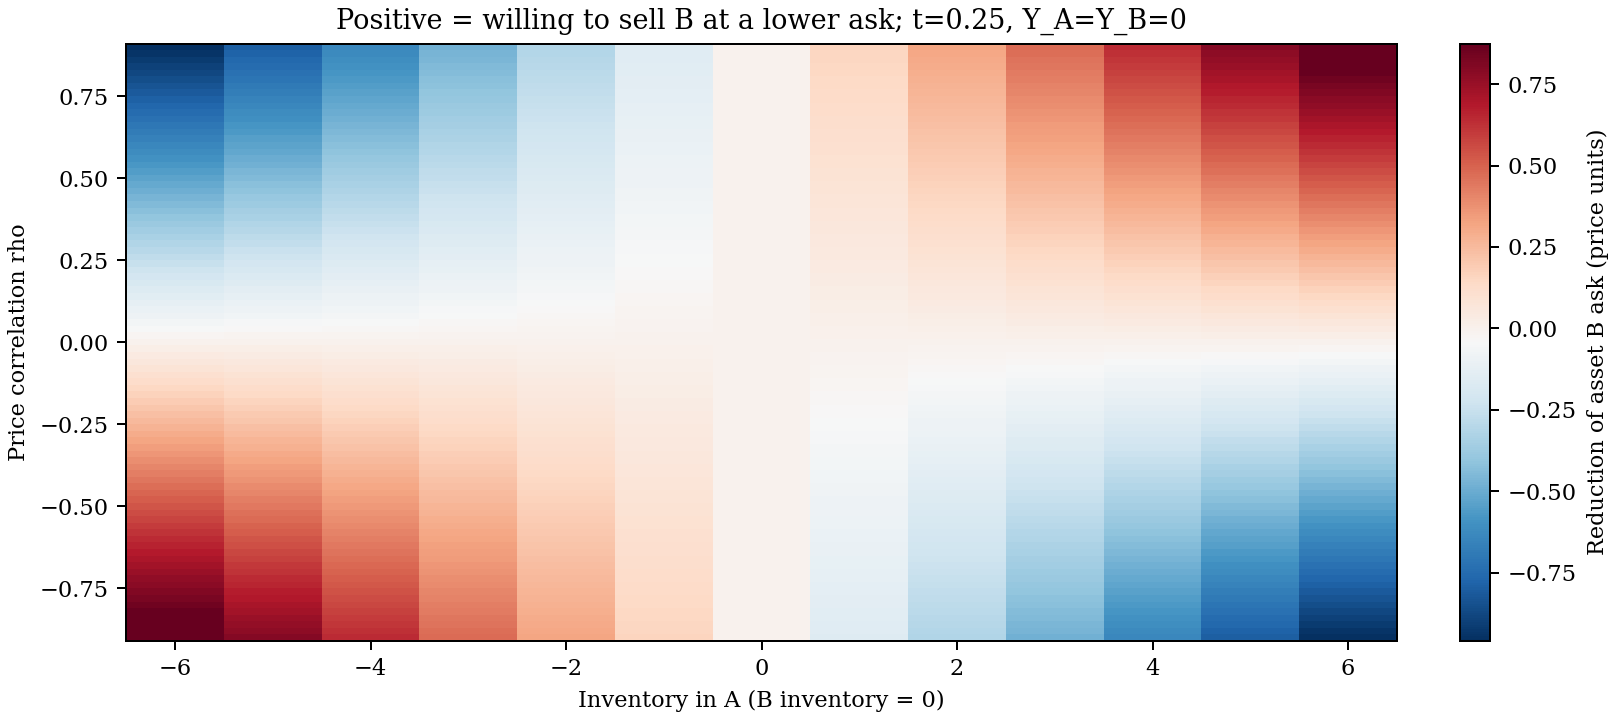
\includegraphics[width=\textwidth]{img/multiasset_quote_shift.png}
\caption{Reduction of asset B's ask relative to the separate policy, with $q_B=0$, $Y_A=Y_B=0$ and $t=0.25$. Positive values indicate a lower ask. The map varies price correlation and A inventory, using actual interpolated baseline gains and bounded controls. Zero correlation removes this explicit correction; negative correlation reverses its direction.}
\label{fig:multi-shift}
\end{figure}

\section{Joint simulations and the risk--revenue trade-off}
Both strategies begin with $q=(3,0)$, prices $(100,100)$ and cash $-300$, so initial marked wealth is zero. This deliberately exposes the cross-asset response to a long A position. For each asset the inventory limit is six units and the arrival parameters remain $A=14$, $k=1.15$. One marked Poisson candidate stream of total rate 56 chooses asset and side uniformly; acceptance probability is $e^{-k\delta}$. Inventory and both assets' quotes are updated after every accepted candidate. Common candidates and exogenous shocks pair the two policies. Price and volatility remain frozen during each interval's arrivals, followed by diffusion updates. All assets are liquidated at $T$ and the sum of the two declared liquidation costs is charged once.

Figure~\ref{fig:multi-inventory} shows path zero under seed 73, fixed independently of the outcomes. Purple B inventory initially becomes short while A is long. Later, when positions and prices have evolved differently, the same policy can carry more risk than the separate policy. The selected path is illustrative; it is not required to exhibit the average ranking at every time.

\begin{figure}[p]
\centering
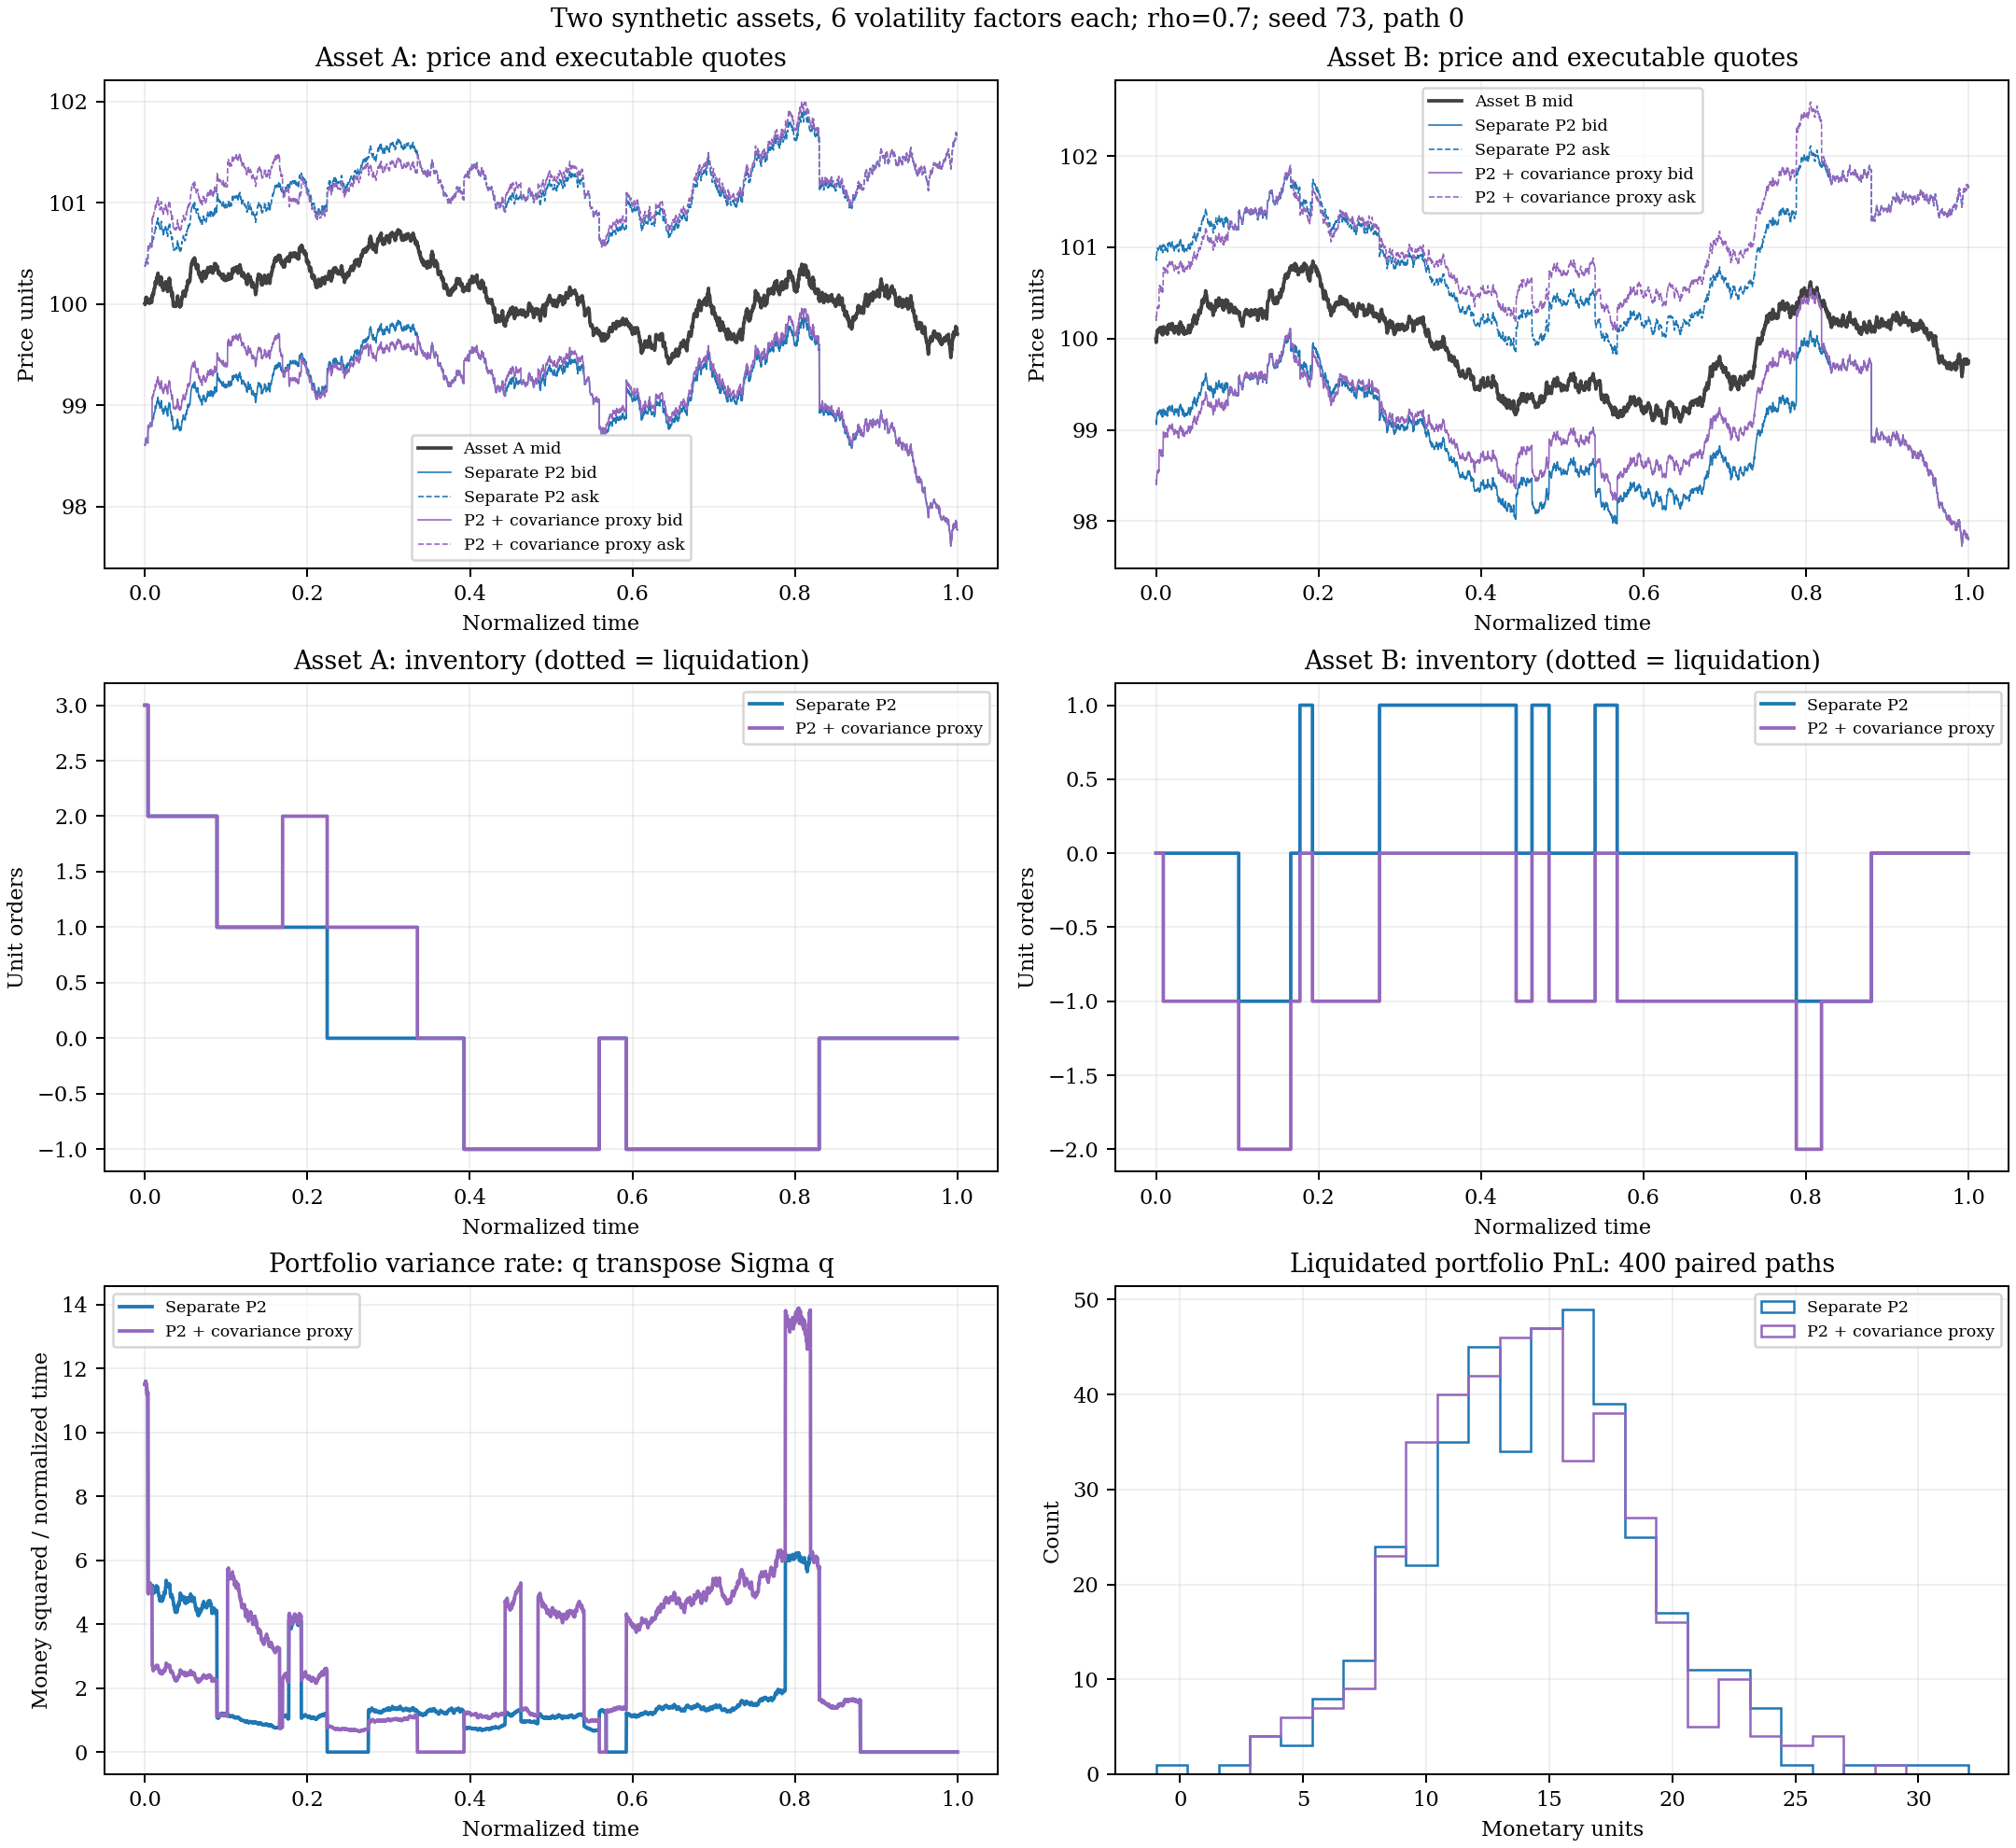
\includegraphics[width=\textwidth]{img/multiasset_inventory.png}
\caption{Two-asset application of separate P2 and P2 plus the covariance proxy. Top: both price paths and executable quotes. Middle: both inventories, with terminal liquidation dotted. Bottom: portfolio variance rate on the fixed illustrative path and liquidated PnL over 400 paired paths. Main run: 3900 intervals, price correlation 0.7, volatility-driver correlation 0.35, seed 73. The proxy is not the fitted residual-corrected policy P3.}
\label{fig:multi-inventory}
\end{figure}

For the main 400-path experiment, the results are
\begin{center}
\begin{tabular}{@{}lrr@{}}
\toprule
Metric & Separate P2 & Covariance proxy\\
\midrule
Mean $\int_0^Tq_t^\top\Sigma_tq_t\,dt$ & 5.8443 & 4.9608\\
Mean liquidated PnL & 14.4335 & 14.0905\\
Sample CARA certainty equivalent & 12.3054 & 12.2345\\
Mean $|q_A|$ before liquidation & 0.5275 & 0.5300\\
Mean $|q_B|$ before liquidation & 0.4825 & 0.5200\\
\bottomrule
\end{tabular}
\end{center}
The integrated-risk difference (proxy minus separate) is $-0.8835$, with paired standard error 0.1085: approximately 15.1\% lower mean integrated variance. This metric measures accumulated instantaneous inventory risk, not the sample variance of terminal PnL. The mean PnL difference is $-0.3430$, with paired standard error 0.0908. The sample certainty equivalent $-\log(\operatorname{mean}e^{-\gamma\mathrm{PnL}})/\gamma$ also decreases slightly; no confidence interval for that nonlinear statistic has been computed. The experiment therefore does not establish an improvement in the CARA objective. It shows a risk--revenue trade-off and motivates a better correction rather than validating this proxy as optimal.

A 1950-interval diagnostic with 400 paths has the same qualitative average trade-off: integrated variance 5.9781 versus 5.2543, PnL 13.9323 versus 13.6632. These two resolutions do not certify convergence. Reusing a seed at a different step count does not couple identical Brownian paths across resolutions; pairing is within each run. A separate zero-price-correlation regression produces identical inventories, cash and outcomes for both policies, even though the volatility drivers retain correlation 0.35. Thus this correction isolates price-covariance inventory coupling, not every source of dependence.

\section{From a covariance proxy to a full residual correction}
The full lifted operator now has two inventory coordinates and twelve volatility coordinates. With $a$ the instantaneous covariance of the factor drivers and $\mathcal L_Z$ their OU generator, price/factor independence gives
\begin{align*}
\mathcal H[\theta]={}&\theta_t+\mathcal L_Z\theta
-\frac{\gamma}{2}(\nabla_Z\theta)^\top a\nabla_Z\theta
-\frac{\gamma}{2}q^\top\Sigma(Z)q\\
&+\sum_{i=1}^{2}\bigl[H_i(\theta(q+e_i)-\theta(q))
+H_i(\theta(q-e_i)-\theta(q))\bigr],
\end{align*}
omitting forbidden transitions. The C++ implementation supports fixed asset and total-factor dimensions and common arrival/control parameters; its caller supplies valid covariance matrices. Tests cover cross-asset risk, mixed factor Hessians, the gradient-square term and inventory bounds. In the restricted constant-covariance, no-arrival setting, the time derivative of $C_{\rm cov}$ exactly cancels the omitted cross-risk term relative to the diagonal baseline. That algebraic check does not establish cancellation in the stochastic-volatility model.

Indeed, $C_{\rm cov}$ also has factor derivatives when $\Sigma$ is stochastic, and changes all arrival Hamiltonians through the neighboring-inventory gains. Correlated volatility drivers introduce further mixed terms. The complete residual must be recomputed with these contributions before a localized fitted correction can be accepted. No residual reduction is asserted for the proxy in the experiment above.

For $N$ assets and $K$ total factors, a tensor inventory grid already contains $(2Q+1)^N$ states before discretizing volatility. Reusing separate scalar policies avoids that joint solve, but loses coupling. The explicit pair correction requires a covariance--inventory product, costing $O(N^2)$ for a dense covariance, in addition to scalar lookups; factor simulation costs are separate. This explains the proposed computational advantage and its approximation cost. No measured speedup is reported. The next research step is to use a validated multi-asset baseline and full residual to fit and test localized corrections, retaining risk, utility and computational cost as distinct acceptance criteria.
\clearpage
